\section{Related work}\label{s:related}
\begin{figure*}
\centering
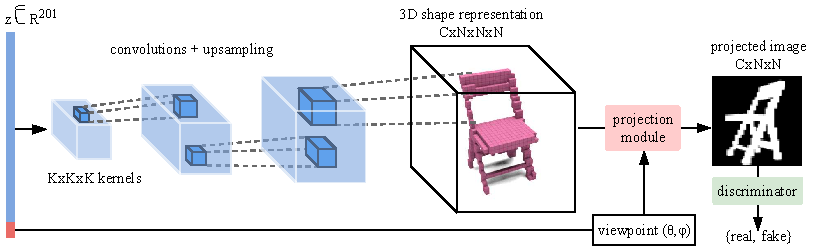
\includegraphics[width=\linewidth]{fig/prgan-arch-fix.pdf}
\caption{\label{fig:prgan-arch} \emph{The PrGAN architecture for generating
  2D silhouettes of shapes factorized into a 3D shape generator and
  viewpoint generator and projection module.} A 3D voxel representation ($\text{C}
  \times \text{N}^3$) and
  viewpoint are independently generated from the input $z$ (201-d
  vector). The projection module renders the voxel shape from a given
  viewpoint $(\theta,\phi)$ to create an image. The discriminator
  consists of 2D convolutional and pooling layers and aims to classify
  if the generated image is ``real'' or ``fake''. The number of
  channels C in the generated shape is equal to one for an
  occupancy-based representation and is equal to the number of parts
  for a part-based representation.}

\end{figure*}


\paragraph{Estimating 3D shape from image collections.} 
The difficulty of estimating 3D shape can vary widely based on how the
images are generated and the assumptions one can make about the underlying
shapes.
Visual-hull techniques~\cite{laurentini1994visual} can be used to
infer the shape of an object by computing the intersection of the
projected silhouettes taken from known viewpoints. 
When the viewpoint is fixed and the lighting is known, photometric
stereo~\cite{woodham1980photometric} can provide accurate geometry
estimates for rigid and diffuse surfaces.
Structure from motion (SfM)~\cite{hartley2003multiple} can be used to
estimate the shape of \emph{rigid objects} from their views taken from
unknown viewpoints by jointly reasoning about point correspondences
and camera projections. 
Non-rigid SfM can be used to recover shapes from image collections by
assuming that the 3D shapes can be represented using a compact parametric model.
An early example is that of Blanz and Vetter~\cite{blanz1999morphable} for
estimating 3D shapes of faces from image collections where each shape
is represented as a linear combination of bases (Eigen shapes). 
However, 3D shapes need to be aligned in a
consistent manner to estimate the bases which can be challenging.
Recently, non-rigid SfM has been applied to categories such as cars
and airplanes by manually annotating a fixed set of keypoints across
instances to provide correspondences~\cite{kar2015category}.
Our work augments non-rigid SfM using a learned 3D shape generator,
which allows us to generalize the technique to categories with diverse
structures \emph{without} requiring correspondence annotations.
Our work is also related to recent work of Kulkarni
\etal \cite{kulkarni2015deep} for estimating a disentangled
representation of images into shape, viewpoint, and lighting variables
(dubbed ``inverse graphics networks"). However, the shape
representation is not explicit, and the approach requires the ability
to generate training images while varying one factor at a time.

\paragraph{Inferring 3D shape from a single image.} Optimization-based
approaches put priors on geometry, material, and light to estimate
all of them by minimizing the reconstruction error when
rendered~\cite{land1971lightness,barrow1978recovering,BarronTPAMI2015}.
Our approach on the other hand exploits implicit priors induced by
deep networks~\cite{deepshapeprior,bayesiandip} for generative modeling.
Recognition-based methods have been used to estimate geometry of
outdoor scenes~\cite{hoiem2005geometric,saxena2005learning}, indoor
environments~\cite{eigen2015predicting,schwing2012efficient}, and
objects~\cite{andriluka2010monocular,savarese20073d}.
More recently, convolutional networks have been trained to generate
views of 3D objects given their attributes and camera
parameters~\cite{dosovitskiy2015learning}, to generate 3D shape given
a 2D view of the object~\cite{tatarchenko2016multi}, and to generate
novel views of an object~\cite{zhou2016view}. Most of these approaches
are trained in a fully-supervised manner and require 3D data or
multiple views of the same object during training.



\paragraph{Generative models for images and shapes.} Our work builds
on the success of GANs for generating images across a wide range of
domains~\cite{goodfellow2014generative}. 
Recently, Wu \etal \cite{wu2016learning} learned a generative model of
3D shapes using GANs equipped with 3D convolutions.
However, the model was trained with aligned 3D shape data.
Our work aims to solve a more difficult question of learning a 3D-GAN
from 2D images. 
Several recent works are in this direction. 
Rezende \etal~\cite{rezende2016unsupervised} show results for 3D
shape completion for simple shapes when views are provided, 
but require the viewpoints to be known and the generative models are
trained on 3D data. 
Yan \etal~\cite{yan2016perspective} learn a mapping from an image
to 3D using multiple 
projections of the 3D shape from known viewpoints and object
identification, i.e., which images correspond to the same object. 
Their approach employs a 3D volumetric decoder and optimizes a loss that measures the 
overlap of the projected volume on the multiple silhouettes from known viewpoints, 
similar to a visual-hull reconstruction. 
Tulsiani \etal~\cite{drcTulsiani17} learn a model to map images to 3D
shape provided with color images or silhouettes of objects taken from
known viewpoints using a ``ray consistency'' approach similar to our
projection module.
Kanazawa \etal~\cite{cmrKanazawa18} employs additional supervision in the form of
keypoint annotations to generate textured 3D meshes.
On the other hand, our method does not assume known viewpoints,
object associations of the silhouettes making the problem considerably
harder.
If object associations are given and viewpoints are unknown, a possible
solution is to use multi-view consistency across similar objects, as demonstrated in~\cite{mvcTulsiani18}.
More similar to our setup, Henderson and Ferrari~\cite{henderson18} propose a method to learn
a generative model of 3D shapes from a set of images without viewpoint supervision.
However, their approach uses a more constrained shape representation -- sets of blocks or deformations
in a subdivided cube -- and other visual cues such as lighting configuration and normals.

\paragraph{Differentiable renderers.} 
Our generative models rely on a
differentiable projection module to incorporate image-based supervision.
Since our images are rendered as silhouettes, the process
can be approximated using differentiable functions composed of spatial
transformations and projections as described in Section~\ref{s:method}. 
However, more sophisticated differentiable renders, such as~\cite{nmr,Liu18,dmc}, that take into
account shading and material properties could provide richer
supervision or enable learning from real images.
These renderers rely on mesh-based or surface-based representations which are
challenging to generate due to their unstructured nature.
Recent work on generative models of 3D shapes with point
clouds~\cite{lin18,mrt,gadelha3d17,psg,atlasnet,latentpc} or multiview~\cite{lun17,tatarchenko2016multi} representations
provide a possible alternative to our voxel based approach that we aim
to investigate in the future.
